% Created 2015-06-14 Dom 17:48
\documentclass[11pt]{article}
\usepackage[utf8]{inputenc}
\usepackage[T1]{fontenc}
\usepackage{fixltx2e}
\usepackage{graphicx}
\usepackage{longtable}
\usepackage{float}
\usepackage{wrapfig}
\usepackage{rotating}
\usepackage[normalem]{ulem}
\usepackage{amsmath}
\usepackage{textcomp}
\usepackage{marvosym}
\usepackage{wasysym}
\usepackage{amssymb}
\usepackage{hyperref}
\tolerance=1000
\usepackage{minted}
\usemintedstyle{perldoc}
\usepackage{tikz}
\usetikzlibrary{decorations.markings}
\tikzstyle{vertex}=[circle, draw, inner sep=0pt, minimum size=7pt]
\newcommand{\vertex}{\node[vertex]}
\author{Alice Duarte Scarpa, Bruno Lucian Costa}
\date{2015-06-23}
\title{Exercício 7.28 (Tardos)}
\hypersetup{
  pdfkeywords={},
  pdfsubject={},
  pdfcreator={Emacs 24.4.1 (Org mode 8.2.10)}}
\begin{document}

\maketitle

\section{Enunciado}
\label{sec-1}

Um grupo de estudantes está escrevendo um módulo para preparar
cronogramas de monitoria. O protótipo inicial deles funciona do
seguinte modo: O cronograma é semanal, de modo que podemos nos focar
em uma única semana.

\begin{itemize}
\item O administrador do curso escolhe um conjunto de $k$
intervalos disjuntos de uma hora de duração $I_1, I_2, \ldots,
      I_k$, nos quais seria possível que monitores dessem suas
monitorias; o cronograma final consistirá de um subconjunto de
alguns (mas geralmente não todos) esses intervalos.
\item Cada monitor então entra com seu horário semanal, informando
as horas em que ele está disponível para monitorias.
\item O administrador então especifica, para parâmetros $a$, $b$ e
$c$, que cada monitor deve dar entre $a$ e $b$ horas de
monitoria por semana, e que um total de $c$ horas de monitoria
deve ser dado semanalmente.
\end{itemize}

O problema é escolher um subconjunto dos horários (intervalos) e
atribuir um monitor a cada um desses horários, respeitando a
disponibilidade dos monitores e as restrições impostas pelo
administrador.


a) Dê um algoritmo polinomial que ou constrói um cronograma
   válido de horas de monitoria (especificando que monitor cobre
   quais horários) ou informa que não há cronograma válido.


b) O algoritmo acima tornou-se popular, e surgiu a vontade de
   controlar também a densidade das monitorias: dado números $d_i$,
   com $i$ entre $1$ e $5$, queremos um cronograma com pelo menos
   $d_i$ horários de monitoria no dia da semana $i$. Dê um
   algoritmo polinomial para resolver o problema com essa restrição
   adicional.

\section{Solução força-bruta}
\label{sec-2}

\subsection{Algoritmo}
\label{sec-2-1}

\subsection{Implementação}
\label{sec-2-2}

\subsection{Complexidade}
\label{sec-2-3}

\section{Solução usando fluxo}
\label{sec-3}

\subsection{Introdução}
\label{sec-3-1}

Queremos modelar esse problema como um problema de fluxo. Para isso
vamos começar com algumas definições de fluxo.

\subsubsection{Definições}
\label{sec-3-1-1}

Uma rede de fluxo é um grafo direcionado $G =
(V, E)$ com as seguintes propriedades:
\begin{itemize}
\item Existe um único vértice \textit{fonte} $s \in V$. Nenhuma aresta entra em $s$.
\item A cada aresta $e$ está associada uma capacidade máxima inteira
$c_e$ >= 0 e uma capacidade mínima $d_e$ >=0.
\item Existe um único vértice \textit{dreno} $t \in V$. Nenhuma aresta sai de $t$.
\end{itemize}

Um fluxo $f$ de s a t é uma função $f \colon E \to R^+$ que associa a cada
aresta $e$ um valor real positivo $f(e)$ tal que:

\begin{enumerate}
\item $\forall e \in E, d_e \leq f(e) \leq c_e$
\item Para todo nó interno $v$:
\[ \sum_{e \text{ chegando em } v} f(e) = \sum_{e \text{ saindo de } v} f(e) \]
\end{enumerate}

$f(e)$ representa o fluxo que vai passar pela aresta $e$. O valor de
um fluxo é o total que parte do fonte $s$, isso é:

$$\label{valor_fluxo} \mathrm{Valor} = \sum_{e \text{ saindo de } s} f(e) $$

Definição de grafo residual.

\subsubsection{Representação}
\label{sec-3-1-2}

Podemos usar programação orientada a objetos para nos ajudar na
representação da rede de fluxo, simplificando o algoritmo.
TODO: explicar a parte de já construir o grafo reverso.

Vamos usar uma classe para representar arestas. Uma aresta tem as
propriedades: vértice de origem, vértice de destino, capacidade
(e reversa e fluxo, talvez)

\begin{minted}[]{python}
class Aresta():
    def __init__(self, origem, destino, capacidade, capacidade_min=0):
        self.origem = origem
        self.destino = destino
        self.capacidade = capacidade
        self.capacidade_min = capacidade_min
        self.reversa = None
\end{minted}

Agora que temos a classe Aresta, vamos usá-la para auxiliar na
representação de uma rede de fluxo também como objeto.

Uma rede de fluxo tem duas propriedades: adjacências, um dicionário
que mapeia cada vértice às arestas que saem dele e fluxo,
representando as arestas do grafo e fluxo, representando\ldots{}
O construtor da classe inicializa as duas propriedades como dicionários vazios.

Vamos precisar dos seguintes métodos na nossa classe RedeDeFluxo:

\begin{itemize}
\item \verb~novo_vertice(v)~: Adiciona o vértice v à rede
\item \verb~nova_aresta(origem, destino, capacidade)~: Adiciona uma nova aresta a
rede. Também cria a aresta reversa.
\item \verb~novo_fluxo(f, e)~: Adiciona um fluxo $f$ à aresta $e$
\item \verb~encontra_arestas(v)~: Retorna as arestas que partem do vértice $v$
\item \verb~valor_do_fluxo(fonte)~: Encontra o valor do fluxo, como definido em \eqref{valor_fluxo}.
\end{itemize}

\begin{minted}[]{python}
class RedeDeFluxo():
    def __init__(self):
        self.adj = {}
        self.fluxo = {}

    def novo_vertice(self, v):
        self.adj[v] = []

    def nova_aresta(self, origem, destino, capacidade):
        aresta = Aresta(origem, destino, capacidade)
        self.adj[origem].append(aresta)

        # Criando a aresta reversa
        aresta_reversa = Aresta(destino, origem, 0)
        self.adj[destino].append(aresta_reversa)

        # Marcando aresta e aresta_reversa como reversas uma da outra
        aresta.reversa = aresta_reversa
        aresta_reversa.reversa = aresta

    def novo_fluxo(self, e, f):
        self.fluxo[e] = f

    def encontra_arestas(self, v):
        return self.adj[v]

    def valor_do_fluxo(self, fonte):
        valor = 0
        for aresta in self.encontra_arestas(fonte):
            valor += self.fluxo[aresta]
        return valor
\end{minted}

\subsection{Modelando o problema com fluxos}
\label{sec-3-2}

Os dois itens do problema podem ser reduzidos a encontrar o fluxo de
valor máximo em um grafo com capacidades mínimas usando construções
semelhantes.

Para o item a), construimos o grafo da seguinte forma:

\begin{itemize}
\item Criamos um vértice $s$ representando a fonte e um vértice $t$
  representando o dreno
\item Para cada intervalo $I_i \in I_1, I_2, \ldots, I_k$ escolhido pelo
administrador, criamos um vértice $v_i$ e uma aresta $e_i$ de
capacidade mínima 0 e capacidade máxima 1 com origem em $s$ e
destino em $v_i$
\item Para cada monitor $T_i \in T_1, T_2, \ldots, T_m$ criamos um vértice
$w_i$. Se o monitor está disponível para dar monitoria no intervalo
$I_j$ criamos uma aresta de capacidade mínima 0 e capacidade máxima
1 com origem em $I_j$ e destino em $w_i$. Para cada monitor também
criamos uma aresta com origem em $w_i$ e destino $t$ de capacidade
mínima $a$ e capacidade máxima $b$.
\item Para garantir que a solução final terá exatamente $c$ horas de
monitoria, criamos uma nova fonte $s'$ e uma aresta de $s'$ a $s$
com capacidade mínima e máxima $c$.
\end{itemize}

TODO: argumentar que soluções para esse problema são equivalentes a
soluções do problema original

O caso com 3 intervalos e 2 monitores (A e B) em que o monitor A está
disponível nos intervalos 1 e 2 e o monitor B está disponível nos
horários 1 e 3 está representado abaixo. Os rótulos
das arestas são da forma capacidade mínima/capacidade máxima. As
arestas sem rótulo tem capacidade mínima 0 e máxima 1.

\[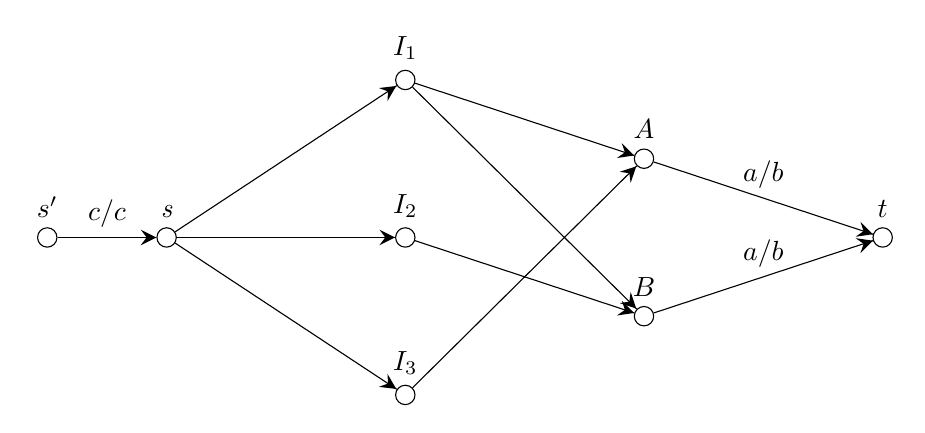
\begin{tikzpicture}[x=0.25\textwidth,
    every edge/.style={
        draw,
        postaction={decorate,
                    decoration={markings,mark=at position 1 with {\arrow[line width = 0.5mm]{stealth}}}
                   }
        }
]
\vertex (fonte') at (0,3) [label=above:$\textit{s}$] {};
\vertex (fonte) at (-0.5,3) [label=above:$s'$] {};
\vertex (I1) at (1,5) [label=above:$I_1$] {};
\vertex (I2) at (1,3) [label=above:$I_2$] {};
\vertex (I3) at (1,1) [label=above:$I_3$] {};
\vertex (A) at (2,4) [label=above:$A$] {};
\vertex (B) at (2,2) [label=above:$B$] {};
\vertex (dreno) at (3,3) [label=above:$t$] {};
\path
(fonte) edge node [above] {$c/c$} (fonte')
(fonte') edge (I1)
(fonte') edge (I2)
(fonte') edge (I3)
(I1) edge (A)
(I1) edge (B)
(I2) edge (B)
(I3) edge (A)
(A) edge node [above] {$a/b$} (dreno)
(B) edge node [above] {$a/b$} (dreno)
;
\end{tikzpicture}\]

\subsection{Implementação}
\label{sec-3-3}

\subsubsection{Fluxo máximo}
\label{sec-3-3-1}

Vamos começar estudando o problema de dada uma rede $G$ em que todas
as capacidades mínimas são iguais a 0, encontrar o fluxo máximo
$f$. Vamos implementar aqui o algoritmo de Ford-Fulkerson para
resolver esse problema.

O algoritmo tem 2 partes:

\begin{enumerate}
\item Dado um caminho $P$ e partindo de um fluxo inicial $f$, obter um
novo fluxo $f'$ expandindo $f$ em $P$
\item Partindo do fluxo $f(e)$ = 0, expandir o fluxo enquanto for possível
\end{enumerate}


\begin{itemize}
\item Primeira parte:
\end{itemize}

O gargalo de um caminho é \ldots{}
Definimos aqui uma função que encontra o gargalo do caminho
\begin{minted}[]{python}
def encontra_gargalo(self, caminho):
    residuos = []
    for aresta in caminho:
        residuos.append(aresta.capacidade - self.fluxo[aresta])
    return min(residuos)
\end{minted}

Expandir o caminho é \ldots{}

\begin{minted}[]{python}
def expande_caminho(self, caminho):
    gargalo = self.encontra_gargalo(caminho)
    for aresta in caminho:
        self.fluxo[aresta] += gargalo
        self.fluxo[aresta.reversa] -= gargalo
\end{minted}

Com isso temos a parte 1 do algoritmo.

Para a parte 2, vamos precisar criar um fluxo $f$ com $f(e) = 0$ para
toda aresta $e$. Podemos fazer isso utilizando o seguinte método na
classe RedeDeFluxo():
\begin{minted}[]{python}
def cria_fluxo_inicial(self):
    for vertice, arestas in self.adj.iteritems():
        for aresta in arestas:
            fluxo[aresta] = 0
\end{minted}

Retorna um caminho de fonte a dreno passando pelos vértices
em caminho
\begin{minted}[]{python}
def encontra_caminho(self, fonte, dreno, caminho):
    if fonte == dreno:
        return caminho
    for aresta in self.encontra_arestas(fonte):
        residuo = aresta.capacidade - self.fluxo[aresta]
        if residuo > 0 and aresta not in caminho:
            resp = self.encontra_caminho(aresta.destino, dreno, caminho + [aresta])
            # TODO: explicar essa parte
            if resp != None:
                return resp
\end{minted}

Com todas as funções auxiliares prontas, podemos finalmente definir a
função que encontra o fluxo máximo.
\begin{minted}[]{python}
def fluxo_maximo(self, fonte, dreno):
    self.cria_fluxo_inicial()
    caminho = self.encontra_caminho(fonte, dreno, [])
    while caminho is not None:
        self.expande_caminho(caminho)
        caminho = self.encontra_caminho(fonte, dreno, [])
    return self.valor_do_fluxo(fonte)
\end{minted}

\subsubsection{Fluxo máximo com capacidades mínimas}
\label{sec-3-3-2}

\subsection{Complexidade}
\label{sec-3-4}
% Emacs 24.4.1 (Org mode 8.2.10)
\end{document}
